

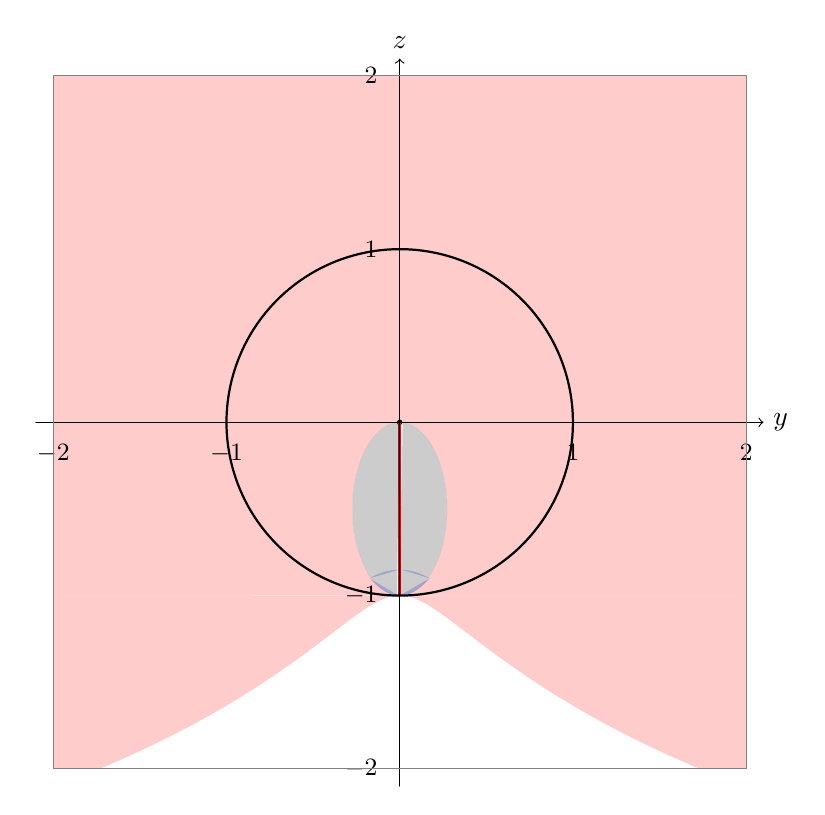
\begin{tikzpicture}[x=2.2cm,y=2.2cm,line join=round,line cap=round]
  % horizontal axis = y, vertical axis = z

  \begin{scope}
    \clip (-2,-2) rectangle (2,2);

    %========================================================
    % Red region: regpl
    %========================================================

    % For 0 <= z <= 2, the whole strip is in the red region
    \fill[red,opacity=0.20] (-2,0) rectangle (2,2);

    % For -1 <= z <= 0: outside the ellipse y^2 = -0.3 z (1+z)
    \fill[red,opacity=0.20]
      plot[domain=-1:0,samples=200]
        ({sqrt(-0.3*\x*(1+\x))},{\x})
      -- (2,0) -- (2,-1) -- cycle;

    \fill[red,opacity=0.20]
      plot[domain=0:-1,samples=200]
        ({-sqrt(-0.3*\x*(1+\x))},{\x})
      -- (-2,-1) -- (-2,0) -- cycle;

    % For -2 <= z <= -1: outside
    % y^2 = -0.3 z^2 (z+1)/(1+0.3 z)
    \fill[red,opacity=0.20]
      plot[domain=-2:-1,samples=200]
        ({sqrt(-0.3*\x*\x*(\x+1)/(1+0.3*\x))},{\x})
      -- (2,-1) -- (2,-2) -- cycle;

    \fill[red,opacity=0.20]
      plot[domain=-1:-2,samples=200]
        ({-sqrt(-0.3*\x*\x*(\x+1)/(1+0.3*\x))},{\x})
      -- (-2,-2) -- (-2,-1) -- cycle;

    %========================================================
    % Black dot shifted to the origin
    %========================================================
    \fill (0,0) circle[radius=1pt];

    %========================================================
    % Red collinear line
    %========================================================
    \draw[red,very thick] (0,0) -- (0,-1);

    %========================================================
    % Soft-collinear region: softCollplot
    % Chosen here in blue (Mathematica default-like extra color)
    %========================================================
    \fill[blue,opacity=0.20]
      (0,-1)
      plot[domain=-1:-0.9,samples=100]
        ({sqrt(0.3*(\x+1))},{\x})
      plot[domain=-0.9:-0.85,samples=100]
        ({sqrt(-0.6*\x-0.51)},{\x})
      plot[domain=-0.85:-0.9,samples=100]
        ({-sqrt(-0.6*\x-0.51)},{\x})
      plot[domain=-0.9:-1,samples=100]
        ({-sqrt(0.3*(\x+1))},{\x})
      -- cycle;

    %========================================================
    % Threshold circle: sqrt(y^2+z^2)=1
    %========================================================
    \draw[thick]
      plot[domain=0:360,samples=240]
        ({cos(\x)},{sin(\x)});

    %========================================================
    % Black collinear region: collregpl
    % y^2 + 0.3 z (1+z) < 0
    %========================================================
    \fill[black,opacity=0.20]
      plot[domain=-1:0,samples=200]
        ({sqrt(-0.3*\x*(1+\x))},{\x})
      plot[domain=0:-1,samples=200]
        ({-sqrt(-0.3*\x*(1+\x))},{\x})
      -- cycle;

  \end{scope}

  %========================================================
  % Axes
  %========================================================
  \draw[->] (-2.1,0) -- (2.1,0) node[right] {$y$};
  \draw[->] (0,-2.1) -- (0,2.1) node[above] {$z$};

  % ticks
  \foreach \t in {-2,-1,1,2}{
    \draw (\t,0.04) -- (\t,-0.04) node[below=2pt] {\small $\t$};
    \draw (0.04,\t) -- (-0.04,\t) node[left=2pt] {\small $\t$};
  }

  % optional plotting window
  \draw[gray] (-2,-2) rectangle (2,2);

\end{tikzpicture}
